%!TEX root = ../PatilM-[RnD-MT]Report.tex
\chapter{Methodology}
\paragraph{}This chapter aims to highlight both the hardware and software setup of the developed system. The integration of the software libraries and packages has been implemented and tested extensively on the `KUKA youBot' which is the aforementioned hardware platform. The following sections briefly illustrate the applied hardware and explain the software packages and their integration with the QSRLib library, which allows us to express physical space qualitatively. 

\section{Hardware Setup}
\paragraph{}The applied robot platform for our application is the `KUKA youBot'. This is an omni-directional platform, equipped with a 5 Degree of freedom robotic arm, that features a two finger gripper. The robot base is equipped with two `Hokuyo URG-04LX' laser range finders situated at the front and at the back respectively, this placement allows for robust localization and map-based navigation in known indoor environments \cite{Roscoe2012}. Physically the dimensions of the robot are as follows length 58cm, width 38cm, height 14cm with a ground clearance of 2cm and a minimum and maximum velocity of 0.01m/s and 0.8m/s respectively \cite{youbot}. The power to this applied platform comes from a 24 volt, 5 Ah lead-acid battery that has an approximate optimal runtime of 90 minutes, but this varies depending upon a multitude of factors such as the robot's velocity, sensors used etc.
\begin{figure}[h]
	\centering
	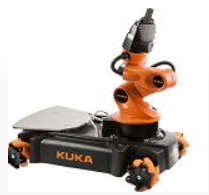
\includegraphics[scale=1]{images/youbot}
	\caption{The youBot robot platform}
	\label{fig:youbot}
\end{figure}

\paragraph{}The robotic arm plays host to a camera mounting which supports the `ASUS Xtion Pro Live' RDB-D camera, which as the name suggests supports the perception of depth information in addition to the usual RGB or raw image data. This RGB-D camera has a detection range of 80cm - 3.5m with a field of view limited to $\ang{58}, \ang{45}, \ang{70}$ horizontally, vertically and diagonally respectively \cite{swoboda2014comprehensive}. The image size for this camera is `640x480' at 30frames per second in a VGA format, also being highly compatible with the `OpenNi development framework' ensures it's easy integration with the ROS packages by the `b-it-bots RoboCup@Work' team, which has already developed scene segmentation and object detection applications centered around this sensor. The stock internal computer that comes issued with the youBot has been replaced with a `Intel Core i5' processor that facilitates highly computational perception tasks to be run directly on the platform \cite{Roscoe2012}. 

\begin{figure}[h]
	\centering
	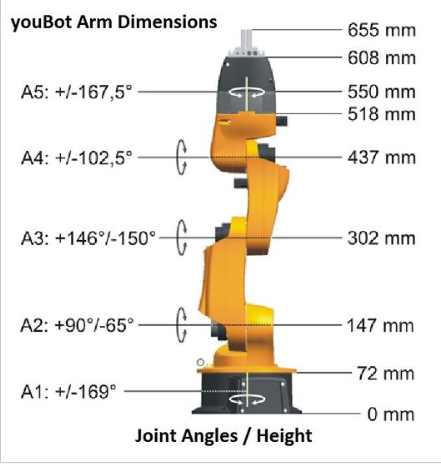
\includegraphics[scale=0.5]{images/youbot_arm}
	\caption{youBot arm at full extension}
	\label{fig:youbotarm}
\end{figure}

\section{Software Framework}
The software framework underpinning the applied robot platform has been developed by the `b-it bots @Work' team and is based on ROS(Kinetic Kame version) or the robot operating system \cite{quigley2009ros}, which provides a modular and distributed structure to design a functional system based on the developer's requirements. This modular architecture provides a rapid and robust communication infrastructure that is based on actions, services and clients to interchange data amongst the various different functional, software components of the applied platform. The framework provides an effective and efficient medium for interfacing various sensors and actuators such as laser scanners, cameras etc. 

\paragraph{}Another merit of the robot operating system is it's provision of advanced tools for visualizing and testing various types of data and troubleshooting the entire system in cases of failures or errors. One such heavily utilized tool was `rosbag', used particularly to capture data \cite{Hegger2012} and evaluate the developed implementation with varying parameters but always on the same set of captured data.

\section{Integration of Qualitative representations}
\paragraph{}The current software framework, set-up on the robot consists of numerous packages that allow the control of it's base as well as arm actuators while also providing an effective interface to it's various sensors. This modular approach facilitates the use of these small components to develop a higher level task. In the instance of `Qualitative spatial representations' we need to access the raw RGB image from the camera to detect features or objects and further extract their approximated pose in order to build a qualitative relation with respect to the robot. The nature of this relation depends upon the type of qualitative calculi that is being implemented in order to define these abstractions.

\paragraph{}As the objective of this project is to show an generalized and efficient utilization of the existing qualitative calculi, we do not develop any of these calculi from scratch, instead deciding to exploit an existing qualitative spatial representations library called `QSRLib' \cite{gatsoulis2016qsrlib}, this library contains ROS compatible  python implementations of the various qualitative calculi, as discussed in the previous chapter. Although this library can be used either as a standalone python package or a ROS catkin package, we use it primarily with ROS and hence shall focus on it's installation and integration with the same. The `qsr\_lib' package is the one that is being used in our implementation and has system dependencies on `numpy' and `matplotlib'. Installing the library is extremely easy as it involves directly cloning the repository(https://github.com/strands-project/strands\_qsr\_lib.git) from git, and moving the `qsr\_lib' package into the `src' folder of our catkin workspace \cite{qsrlib}. 

\paragraph{}The pre-requisites for using any of the qualitative calculi implemented in the library \cite{qsrlib}, \cite{gatsoulis2016qsrlib} is input data such as distinctive object id's or names for the various objects amongst which a qualitative relation is desired, a time-series of the states of the perceived objects and the Cartesian coordinates for each of the objects at every instance of the time series. This information is packaged into a custom input data object that is the default input data format of the library. Additional information such as the size of the object may also be included in the input data object, but it is mandatory to include the name of the qualitative calculi for which the qualitative spatial relations are to be computed. This input data structure is sent to a QSRLib service in the form of a request message, the server then computes the relationships and send the output in the form of a response message(client-service architecture in ROS) that details the qualitative relations between the objects constrained by their respective time stamps. The library comes built with the necessary functions that can be used to convert raw data into the data structure format required by the library. The output of the QSRLib can then be further inspected and employed to make decisions regarding the movement or path of the applied mobile platform.

\begin{figure}[h]
	\centering
	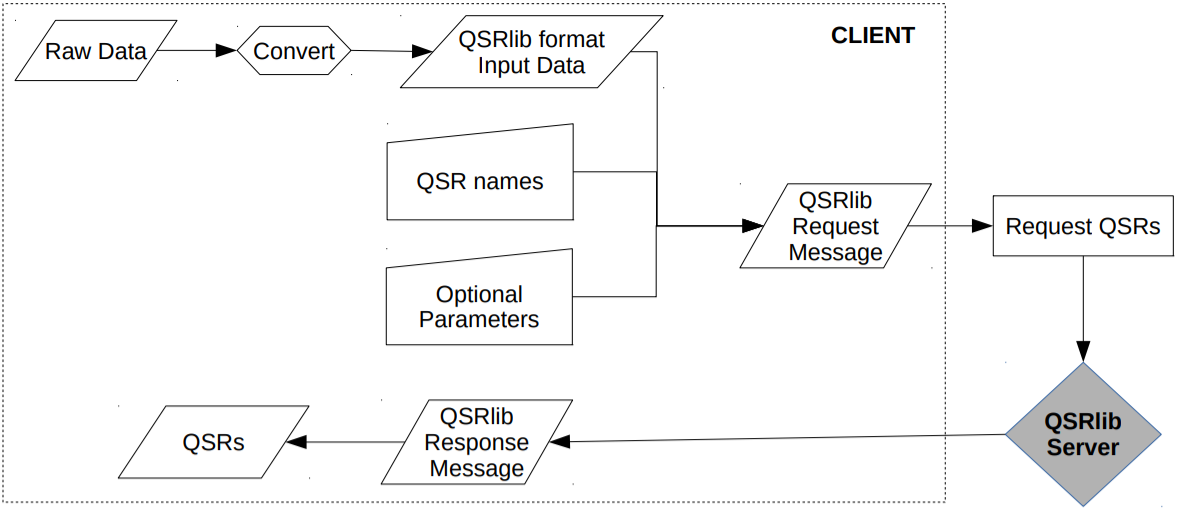
\includegraphics[scale=0.7]{images/qsrlib_flow}
	\caption{A flow chart detailing the inner workings of the QSRLib library \cite{qsrlib}, \cite{gatsoulis2016qsrlib}.}
	\label{fig:qsrlibflow}
\end{figure}


%\section{Use Cases}
%\paragraph{} The main aim of this project is to evaluate the efficiency paradigm of qualitative spatial representations for navigation in mobile robots, especially in closed indoor spaces where quantitative representations of the physical space are considered excessive and unnecessary. Therefore keeping in mind these preconditions we define the following possible use cases.
%
%\subsubsection*{Use case: Navigating in a corridor environment} 
%\paragraph{} A mobile robot is tasked with navigating from point `A' to point `B' in a corridor environment such that it should avoid collision with the walls and any other static or dynamic obstacles if they exist in it's path. Furthermore the robot's movement should be such that it avoids any sudden motions that may seem unsafe or unintuitive to an human agent who might interact with the robot. Also chiefly, the robot must achieve this path traversal in a manner that is as efficient as possible ,while dealing with imprecise information about the environment or in extreme cases lack of complete information about the environment. 
%
%\subsubsection*{Resulting Requirements}
%\paragraph{} Ideally it is desired that any new functionality that is being implemented must be highly generalizable, but keeping in mind the given problem it is unrealistic to expect a `one size fit's all' implementation that works impeccably for all imaginable situations without any restrictions or compromises. Hence a list of requirements resulting from the problem statement and the above described use case is presented below:
%
%\begin{itemize}
%	\item The starting position should be irrelevant when navigating the corridor.
%	
%	\item The detection of the markers or features should be robust with respect to a reasonable speed of the robot.
%	
%	\item The number of markers or features should not adversely affect the robot's behavior. 
%	
%	\item The camera used should have a reasonable field of view so that it can see both the walls and their respective features at any given point of time.
%	
%	\item The camera should be able to capture the features reasonably well, irrespective of the lighting conditions.
%	
%	\item The motion profile of the robot should be a smooth and not disruptive. 
%	
%	\item It should be able to navigate any corridor irrespective of it's size or the color of it's walls.
%\end{itemize}

